%! TEX root = ./master.tex

\lecture{22}{Week: 12}{Large Pages}

\subsubsection{Large Pages}
Sometimes, we want pages which are larger than $4$KB. In that case we want pages of $2$ MB size, we use large pages or if we want pages of $1$ GB size we can use huge pages. All the hardware for larger pages is already there. We simple stop the page walk earlier.

For large pages, it skip the page table table 1 and go do memory using the address obtained from the page directory table.

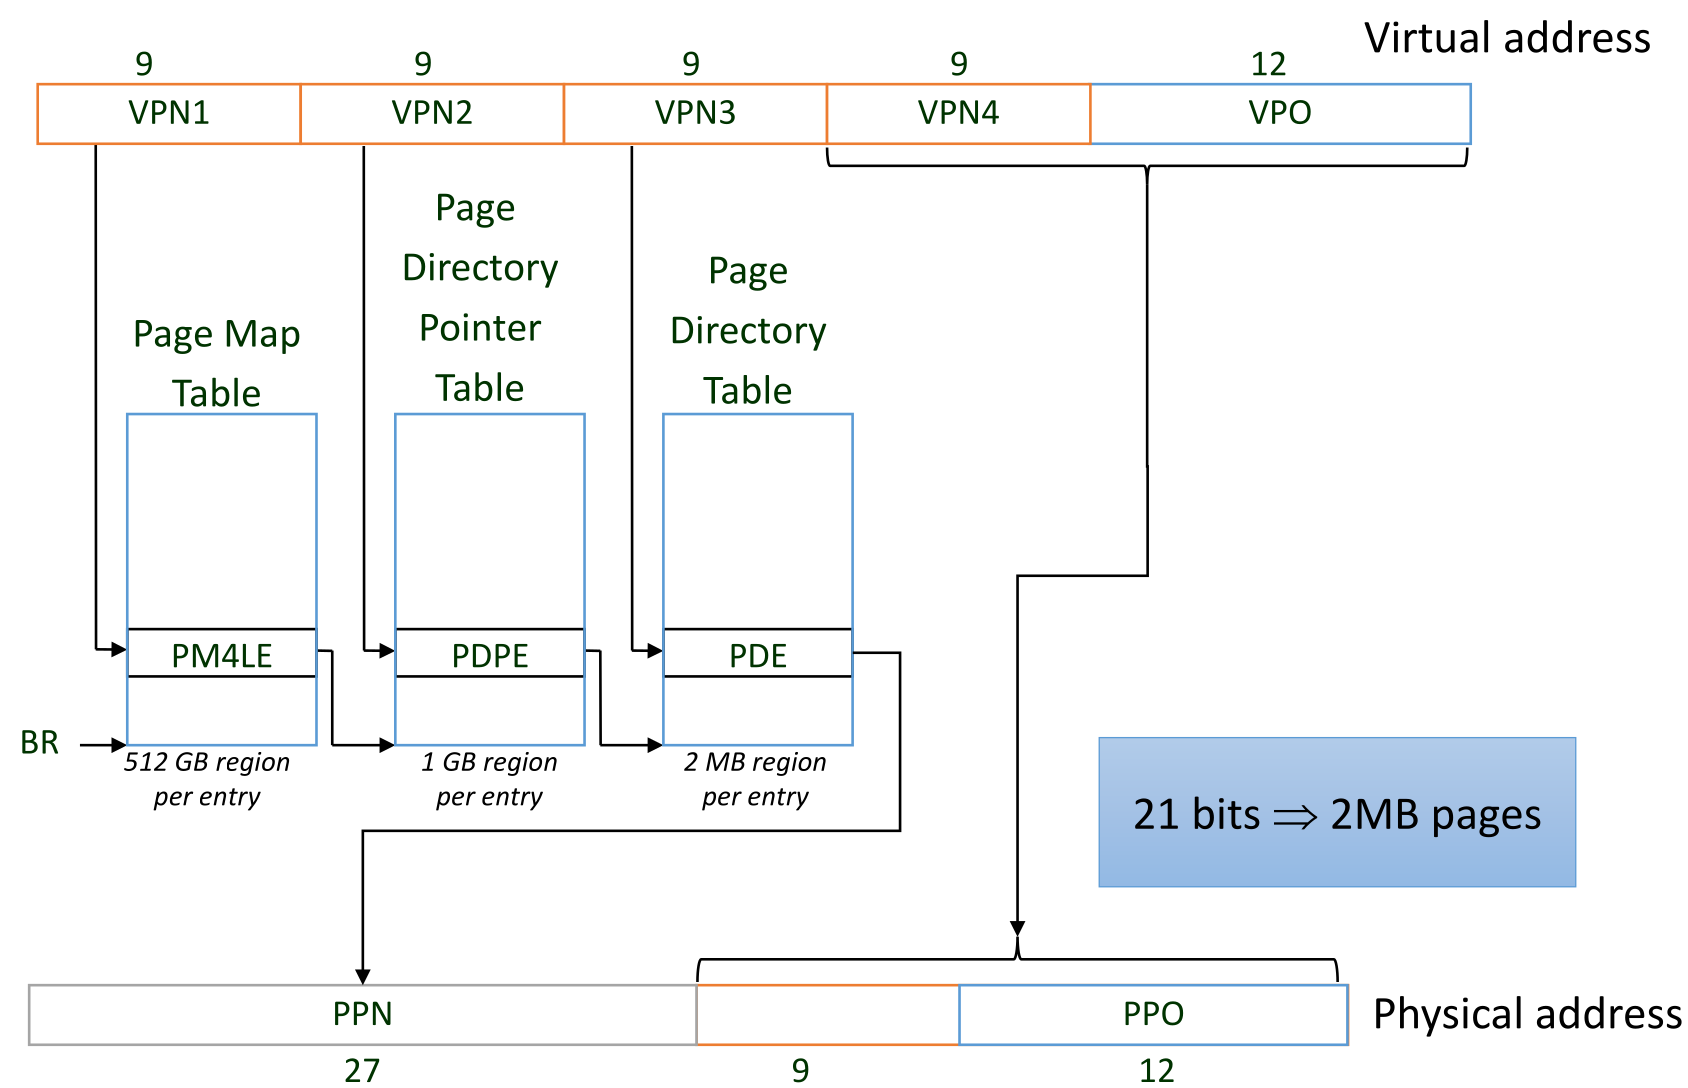
\includegraphics[width=0.8\textwidth]{22_largePage.png}

For huge pages, we skip additionally the page directory table.

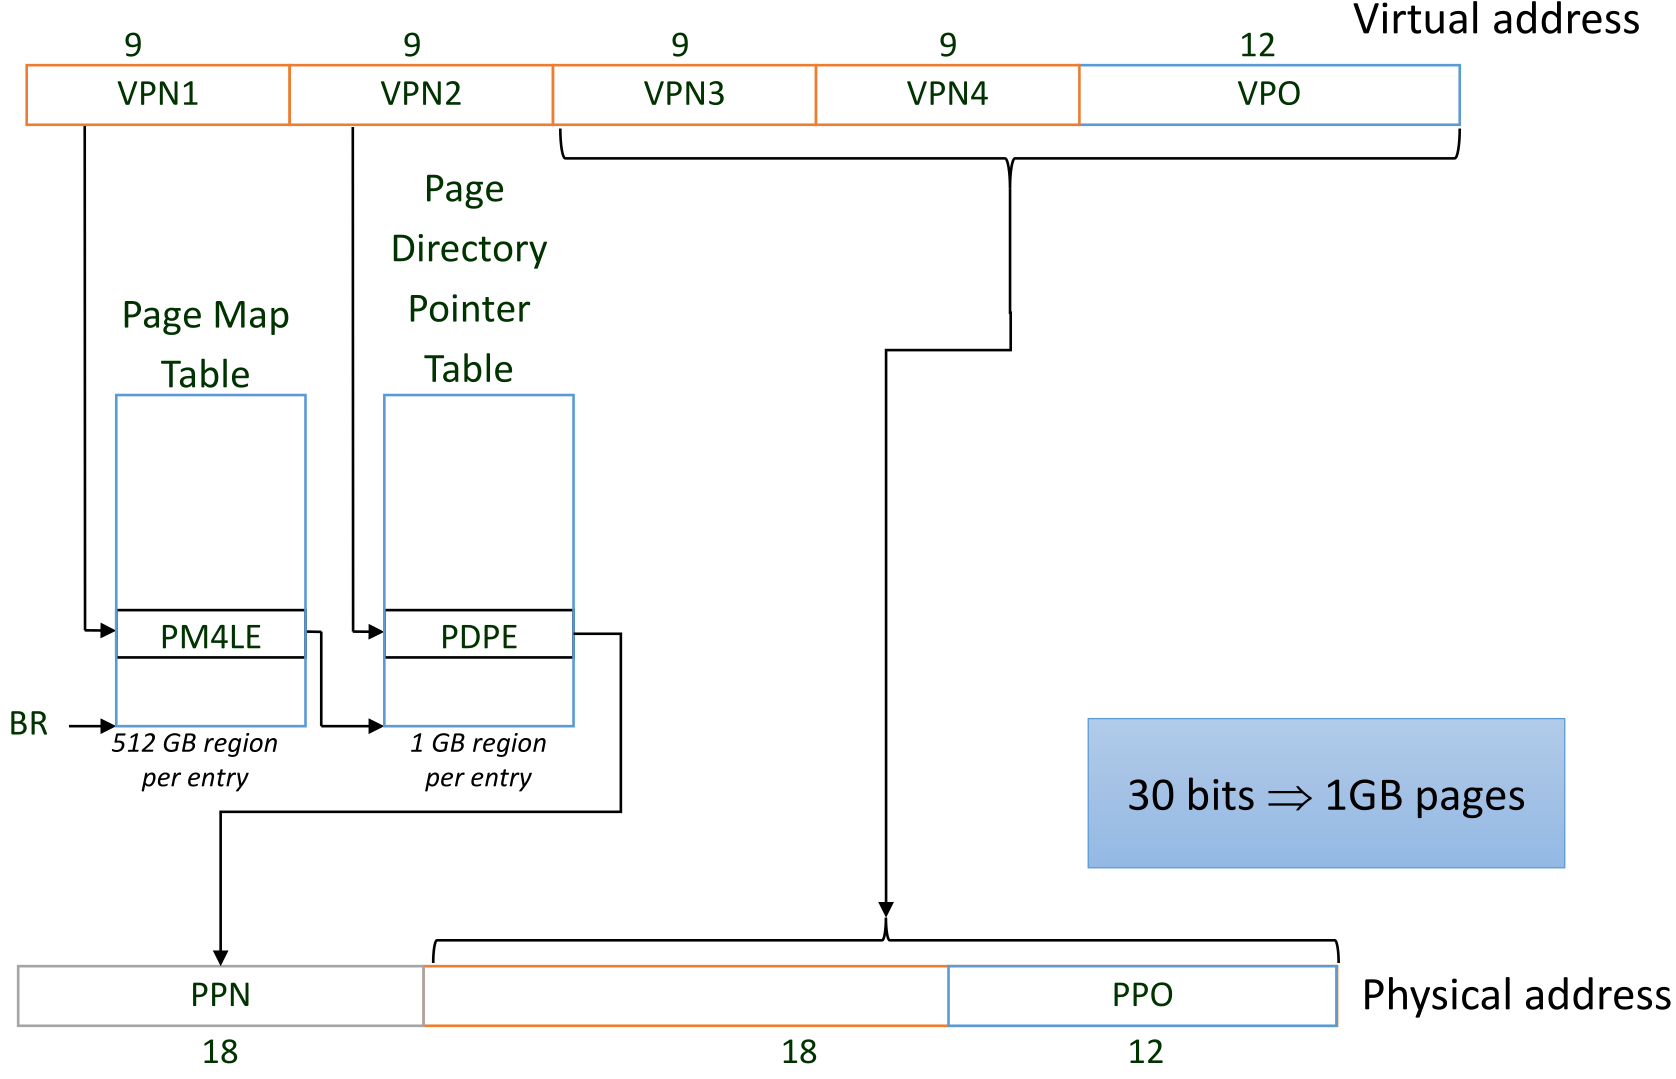
\includegraphics[width=0.8\textwidth]{22_hugePage.png}

Some of the bits of the last table (page directory table for large pages, page directory pointer table for huge pages) need to be changes to represent the dirty bit as well as the global flap.

For large pages:

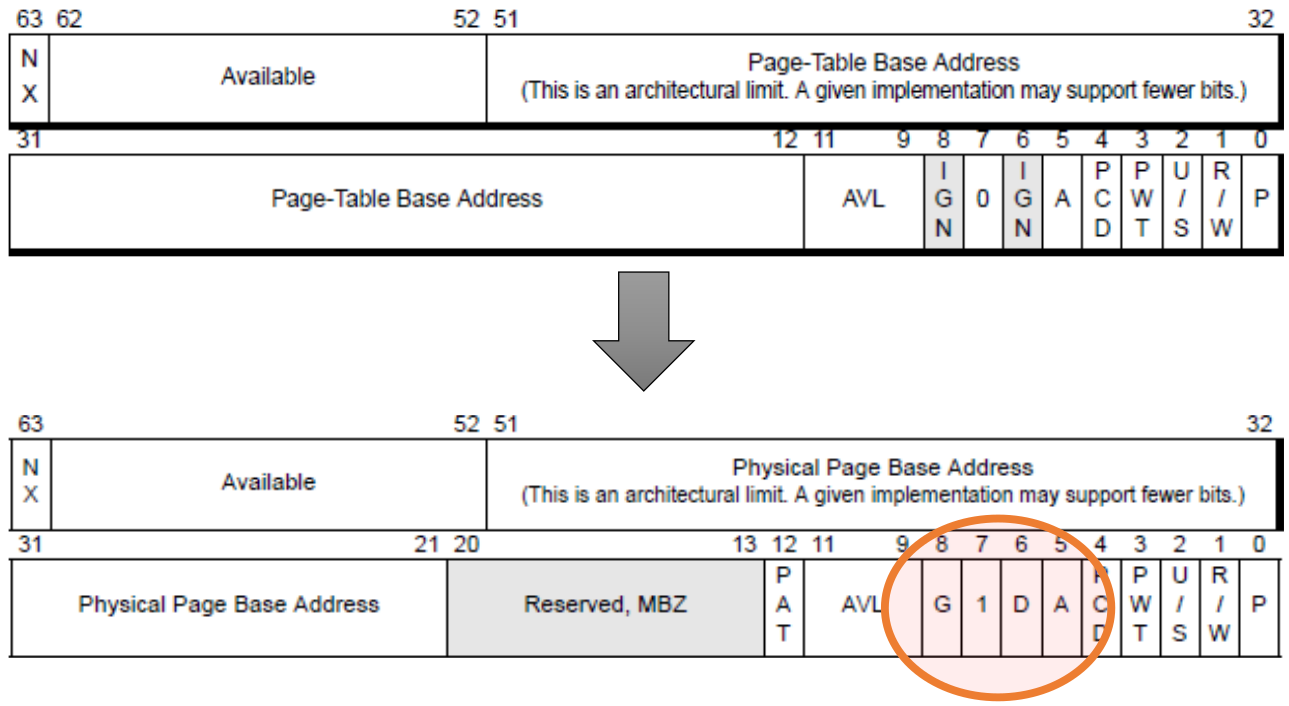
\includegraphics[width=0.8\textwidth]{22_largePageEntry.png}

and for huge pages:

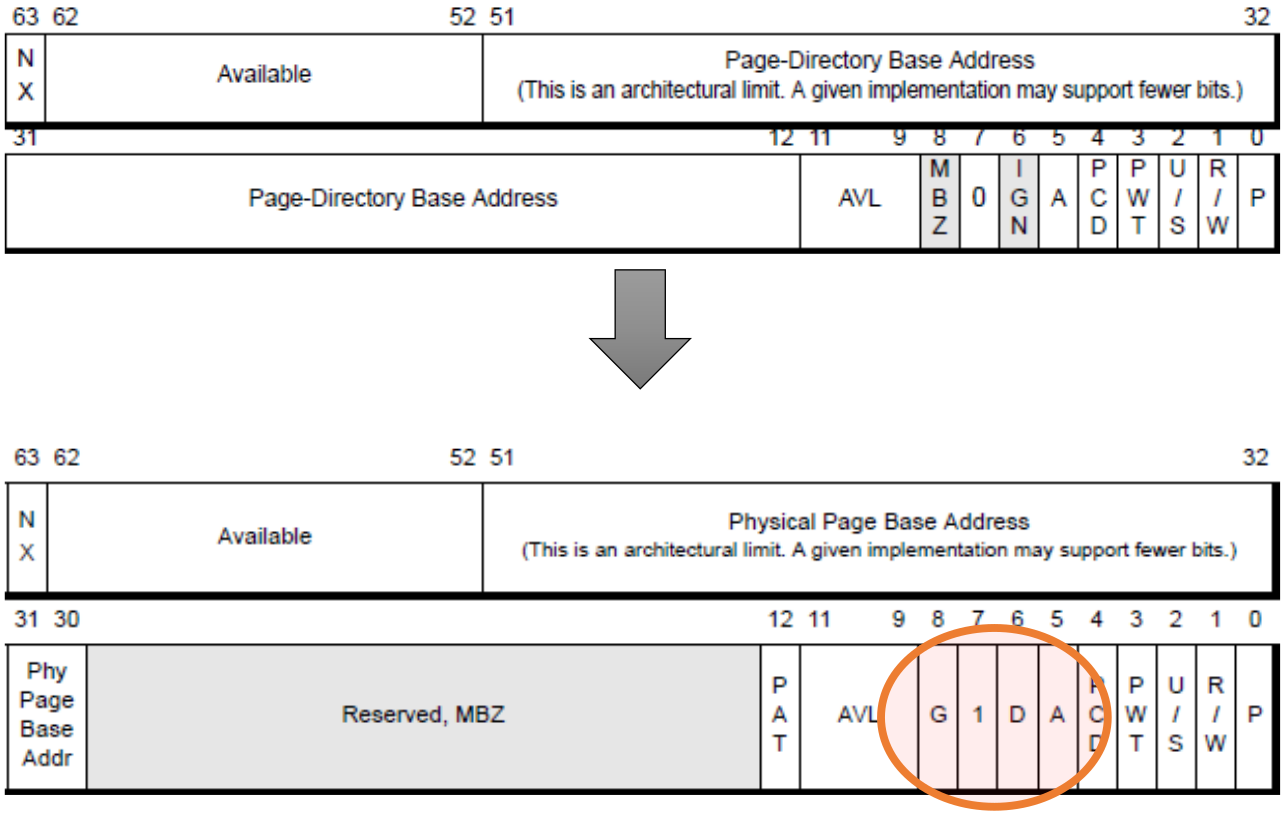
\includegraphics[width=0.8\textwidth]{22_hugePageEntry.png}

All in all, this simplifies and speeds up the address translation. This is very useful for programs with very large, contiguous working sets. Since the TLB is very small, reducing the number of pages increases the hit rate of the TLB. CPUs can do deal with different page sizes in parallel. In Linux, \code{hugetlbfs} is uses for support of larger tables and they get mounted like a regular file system.

\subsubsection{Optimizing for the TLB}
Beside caches, we also need to consider the TLB when optimizing code. Lets assume we want to do matrix multiplication followed by a matrix addition.

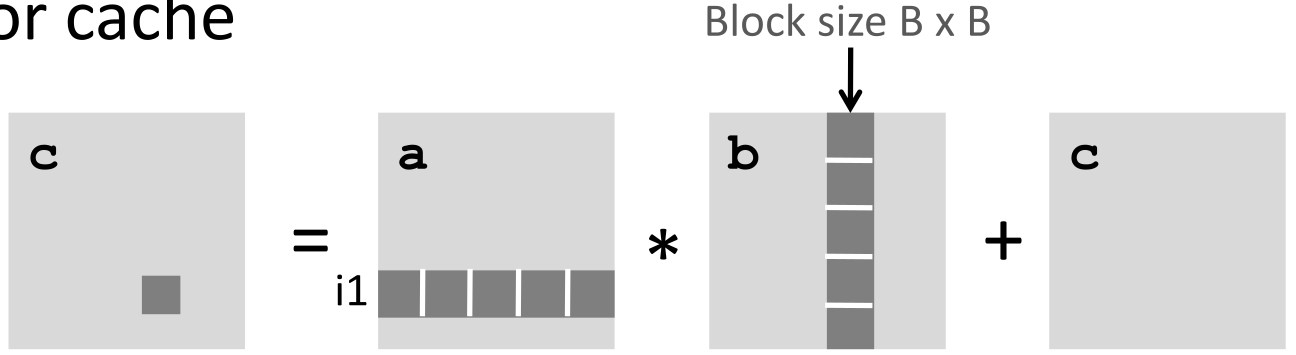
\includegraphics[width=0.8\textwidth]{22_mmm.png}

Let's say we optimize for the L2, which is $16 \text{MB} = 2^{24} = C$. It can store $2^{21}$ doubles. So to optimize for cache and we want to cache the $B \times B$ for matrix a, b, c. So we have $3B^2 < C$ which gives us $B \approx 800$.

But if a block has $800$ rows of size $8$ bits each (i.e. $6400$ bits) is larger than a page size. Therefore, each row is on two pages and then we have this for $800$ rows. This again, we have for the three matrices. The number of pages of a working set is $800 \cdot 2 \cdot 3 = 4800$ pages. That is a lot more than will fit the TLP. 

Just looking at L2 blocking at this size looks ideal, but it is not for the TLB. It will cause TLB thrashing. To prevent this, it makes since the shrink the size of a block and copy the contents of each blocks into a contiguous region of memory to make them fit into a small enough number of page such that they can be hold in the TLB.

We assume a TLB size of $128$ size. If $B = 150$ and the copy the content into a contiguous region of a memory we have a contiguous region of memory of size $150 \cdot 150 \cdot 8 \cdot 3$ bytes. Divided by $4$ KB gives about $128$ tage, which will fit into the TLB. Even though the copying cost $O(B^2)$ we do $O(B^3)$ operations on them. We also need extra space.

\subsection*{Multiprocessing}
\subsubsection{Introduction}
We are all aware of Moore's law; the number of transistors in a circuit doubles every two year, which is thanks to smaller components, which leads to higher clock speeds. But this has changes and therefore we need more cores.

\paragraph{Power Wall}
The power dissipation is $P_{\text{Dynamic}} + P_{\text{Leakage}} + P_{\text{Short}}$

\subparagraph{Dynamic Power}
Used to be the main component. Now it is about $50\%$. It is causes by switching. It is equal $CV^2f$, where $C$ is the capacitance $V$ the supply voltage and $f$ the processor frequency. According to Moore's law, $C$ and $V$ went down, so we could increase $f$ for free. But today, $C$ does not decrease. Decreasing $V$ increases $P_{\text{Leakage}}$ and increasing $f$ increases the power dissipation.

Cooling is an issue too, we have pretty much reached the limit for cooling.

\paragraph{Memory Wall}
The memory call says that the CPU speed increases much faster than the memory bandwidth. This causes memory assesses to get more and more expensive.

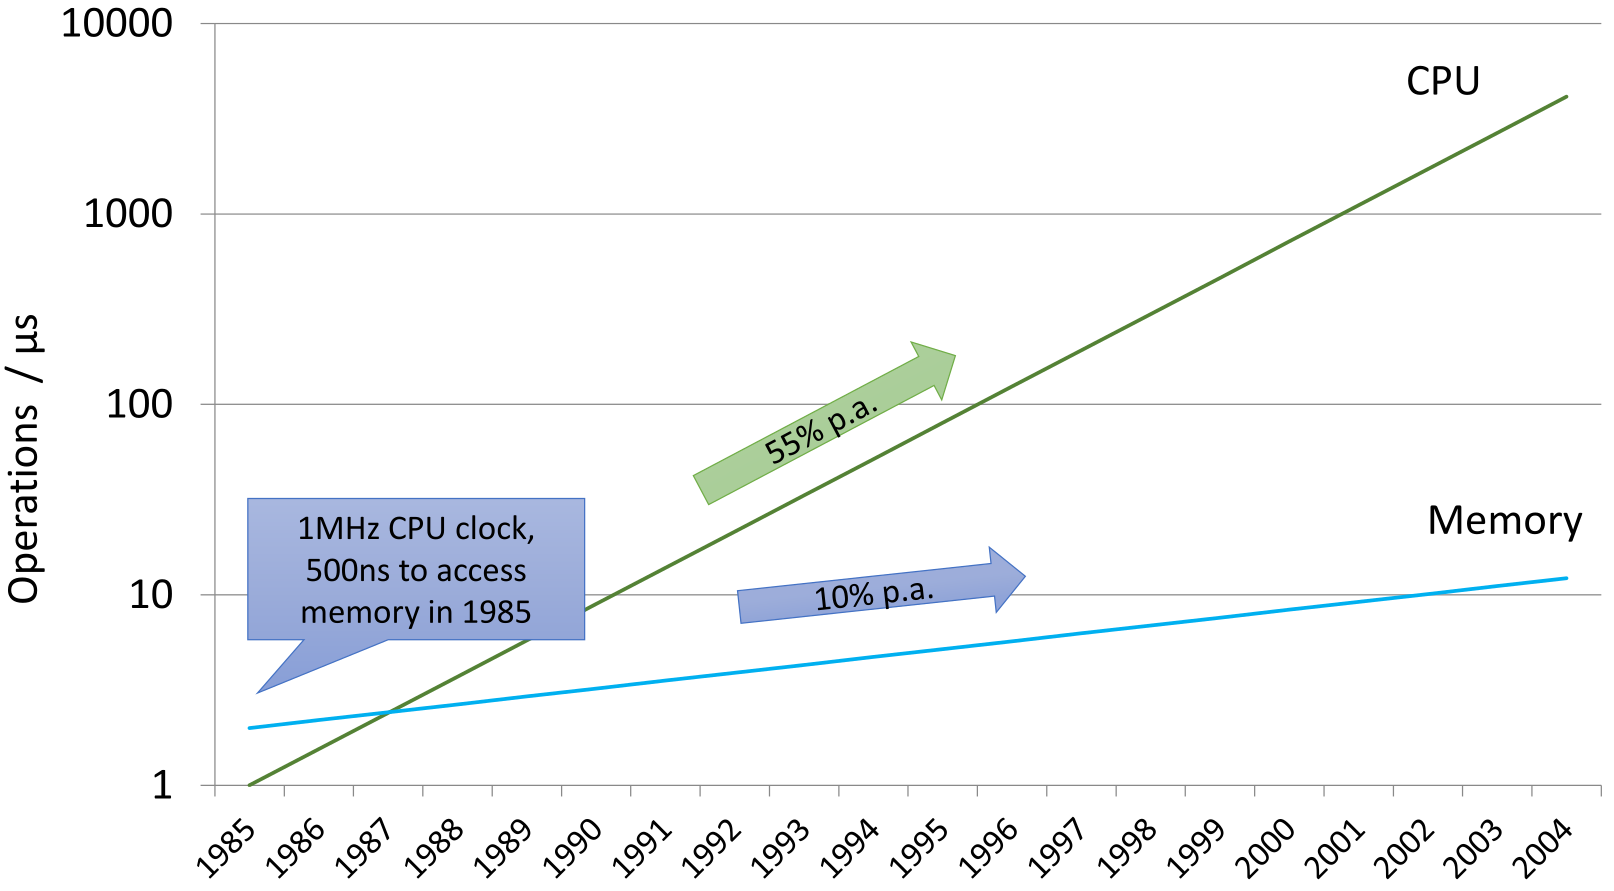
\includegraphics[width=0.8\textwidth]{22_memoryWall.png}

\paragraph{Instruction Level Parallelism (ILP) Wall}
We can do super scalar execution, branch prediction, specular execution to increase ILP. But as we add more transistors, the returns we get are diminishing. A reason for that is that we cannot extract more parallelism from a program than there exists.

\paragraph{Wall Summary}
\begin{itemize}
    \item Power wall: cannot clock processors any faster
    \item Memory wall: often, memory access dominates the performance
    \item ILP wall: cannot keep functional units busy while waiting for memory
\end{itemize}

\paragraph{Multicore Processors}
Multicore CPUs have multiple processor cores on a single CPU chip. Most such CPUs have a single physical address space, which is shared among all processors. The cores communicate though shared variables in memory. This is called \textit{shared memory multiprocessors}.

It is also refered to as symmetric multiprocessing (SMP).

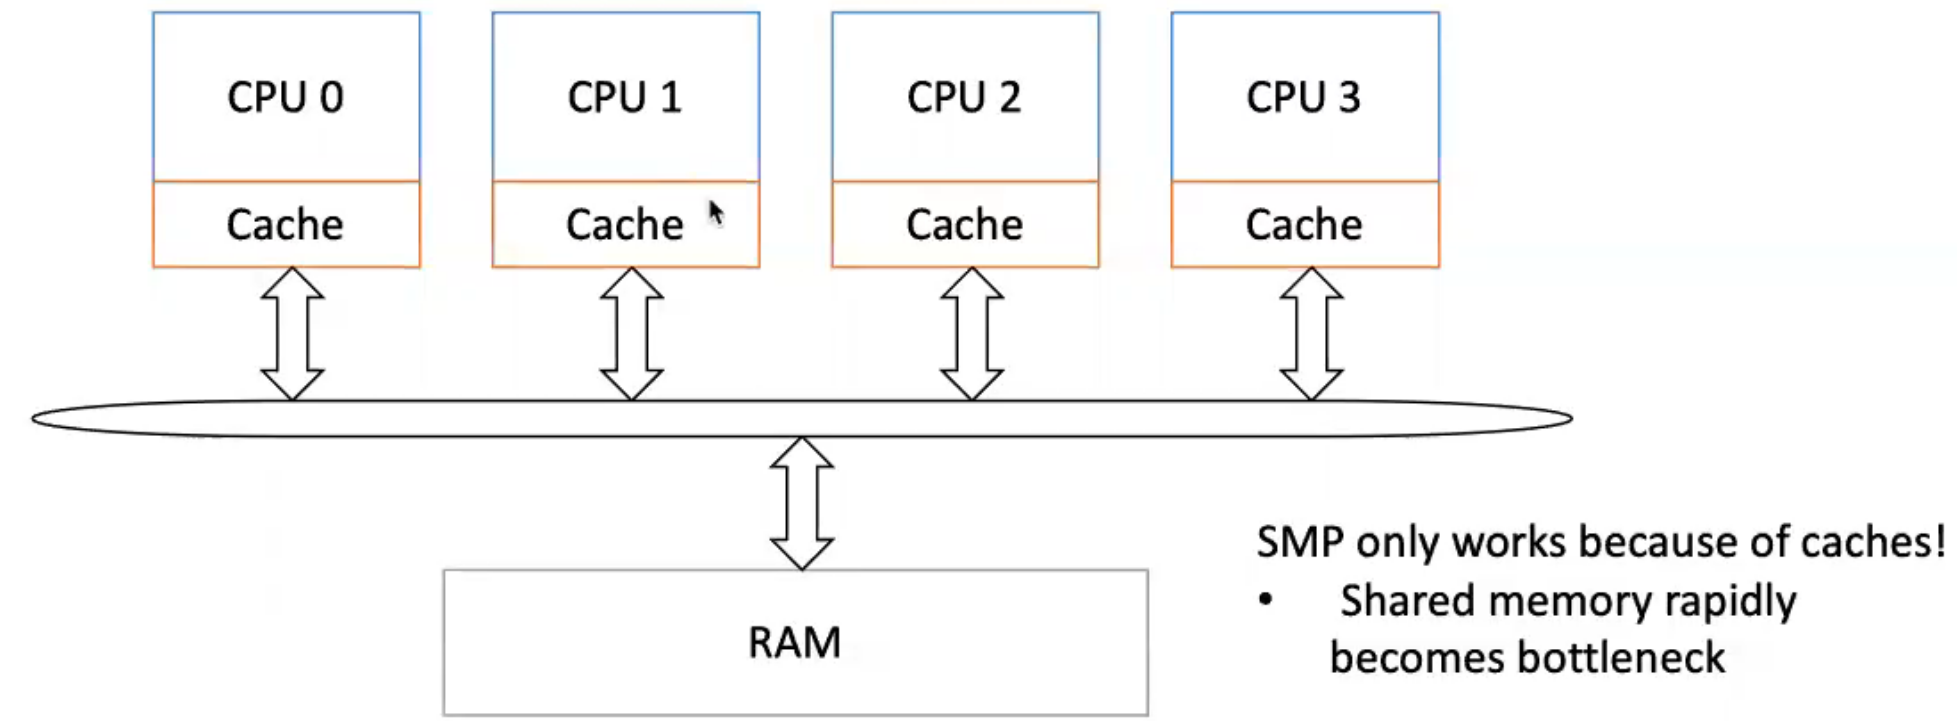
\includegraphics[width=0.8\textwidth]{22_Smp.png}

One major difficulty is how we ensure that all processors have the same view on memory even though hall have their own caches. This is called \textit{cache coherence}.

\subsubsection{Coherency and Consistency}

\paragraph{Coherency}
Cache coherency is about the view on memory by all processors. It means that even though all processors have the same cache, they need a coherent view of memory. I.e. all processors must see the same data on a certain memory location. Most modern CPUs are actually cache coherent. 

The main advantage of this s the ease of programming. But is it more complex to implement.

\paragraph{Consistency}
Memory consistency is the order in which changes to memory are soon by different processors. It is impotent to to have a clear definition.

\subparagraph{Program Order}
Program order is the order in which a program on a processor appear to issue read and writes. It only referees to local read and writes, since it is what is seen by other processes. But the CPU my rearrange other instructions (out-of-order execution, write buffers etc.).

\subparagraph{Visibility Order}
Visibility order it the order in which all reads and writes are seen by other processors. It referees to all operations in the machine. Different processors may have a different visibility order.This means that each processor reads the value written by the last write in visibility order.

\subsubsection{Sequential Consistency}
It is conceptionally the simplest consistency model. Operation from a processor appear to all other processors in program order. And all processors see (visibility order) the same interleaving of the program orders of the different processors. I.e. the visibility order of each processor is the same.

\paragraph{Requirements}
This requires:
\begin{itemize}
    \item each processors issues memory ops in program order (i.e. each processor obeys their program order)
    \item RAM orders all operations is receives in the order it receives them (it has a total order)
    \item memory operations are atomic
\end{itemize}

\paragraph{Example}
\subparagraph{Ex1}
Given two CPUs, A and B, where A writes two variables and B reads these variables. Initially, all variables are $0$.

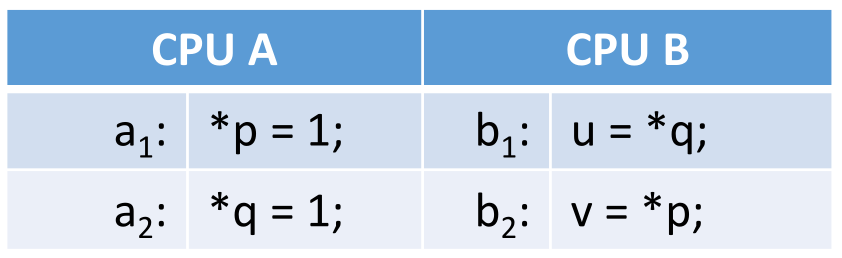
\includegraphics[width=0.8\textwidth]{22_sequentialConsistencyEX.png}

A valid outcome in SC is \code{u=1, v=1}, received when A has program order \code{a1, a2} and B has \code{b1, b2} and the interleaving is \code{a1, a2, b1, b2}.

Could we get \code{u=1, v=0} in SC? We see that this is not possible since \code{a2 > b1 > b2 > a1} which does not respect program order of the processors.

\subparagraph{Ex2}
Given two CPUs, A and B, where both processors first write a variable and then read a variable. Initially, all variables are $0$.

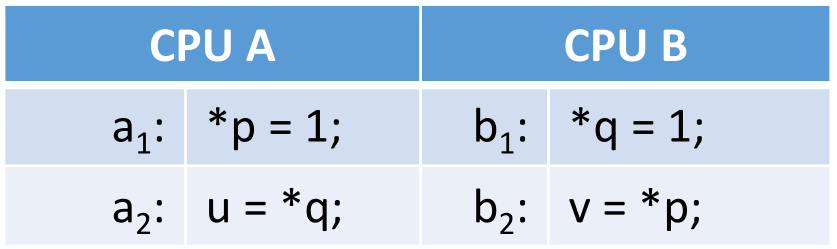
\includegraphics[width=0.8\textwidth]{22_sequentialConsistencyEx2.png}

A valid outcome in SC is \code{u=1, v=1}, received when A has program order \code{a1, a2} and B has \code{b1, b2} and the interleaving is \code{a1, b1, a2, b2}.

Could we get \code{u=1, v=0} in SC? We see that this is not possible since \code{a2 > b1 > b2 > a1} which does not respect program order of the processors.

\paragraph{Advantage / Disadvantage}
\begin{itemize}
    \item Advantage:
        \begin{itemize}
            \item Easy to understand for the programmer
            \item Easy to write correct to to
            \item Easy to analyse automatically
        \end{itemize}
    \item disadvantage:
        \begin{itemize}
            \item Hard to build fast implementation
            \item Cannot reorder reads/writes (even in the compiler or single processors)
            \item Cannot combine writes to same cache line (write buffer)
            \item Serializing operations at memory controller is too restrictive
        \end{itemize}
\end{itemize}

\subsubsection{Cache Coherence With Snooping}
How do we ensure a coherent view of memory. Snooping is a possible solution. \textit{Snooping} is the act on listening on the bus for reads/writes of other processors. If we have a local copy of a cache line and a other processors writes the same line, we invalidate our local cache line. But for this to work, caches must be write-through (else memory is not directly updated on a write and hence, we do not get notified). Obviously, multiple processors can have the same cache line in cache.

\paragraph{Write-Back Caches}
For the snooping to work out of the box, we need write-through caches. Though, often systems have write-back caches two and now cache liens can be dirty. For this to work, we need a \textit{cache coherency protocol}.

\subsubsection{MSI}
A cache line can be in one of three states:
\begin{itemize}
    \item \textit{Modified}: we have changed the cache block (it is dirty)
    \item \textit{Shared}: we read it and there are possible other readers
    \item \textit{Invalid}: we have not cached this line
\end{itemize}

The state we are in depends on

\begin{itemize}
    \item the action we take
    \item what we hear on the bus (i.e. actions of other processors on the same cache line).
\end{itemize}

\paragraph{Invariants}
The MSI invariants are:

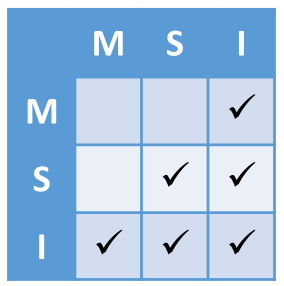
\includegraphics[width=0.8\textwidth]{22_MsiInvariant.png}

\paragraph{Transitions}
We can have the following transitions. Grey are local operations by us, orange remote operations by other processors.

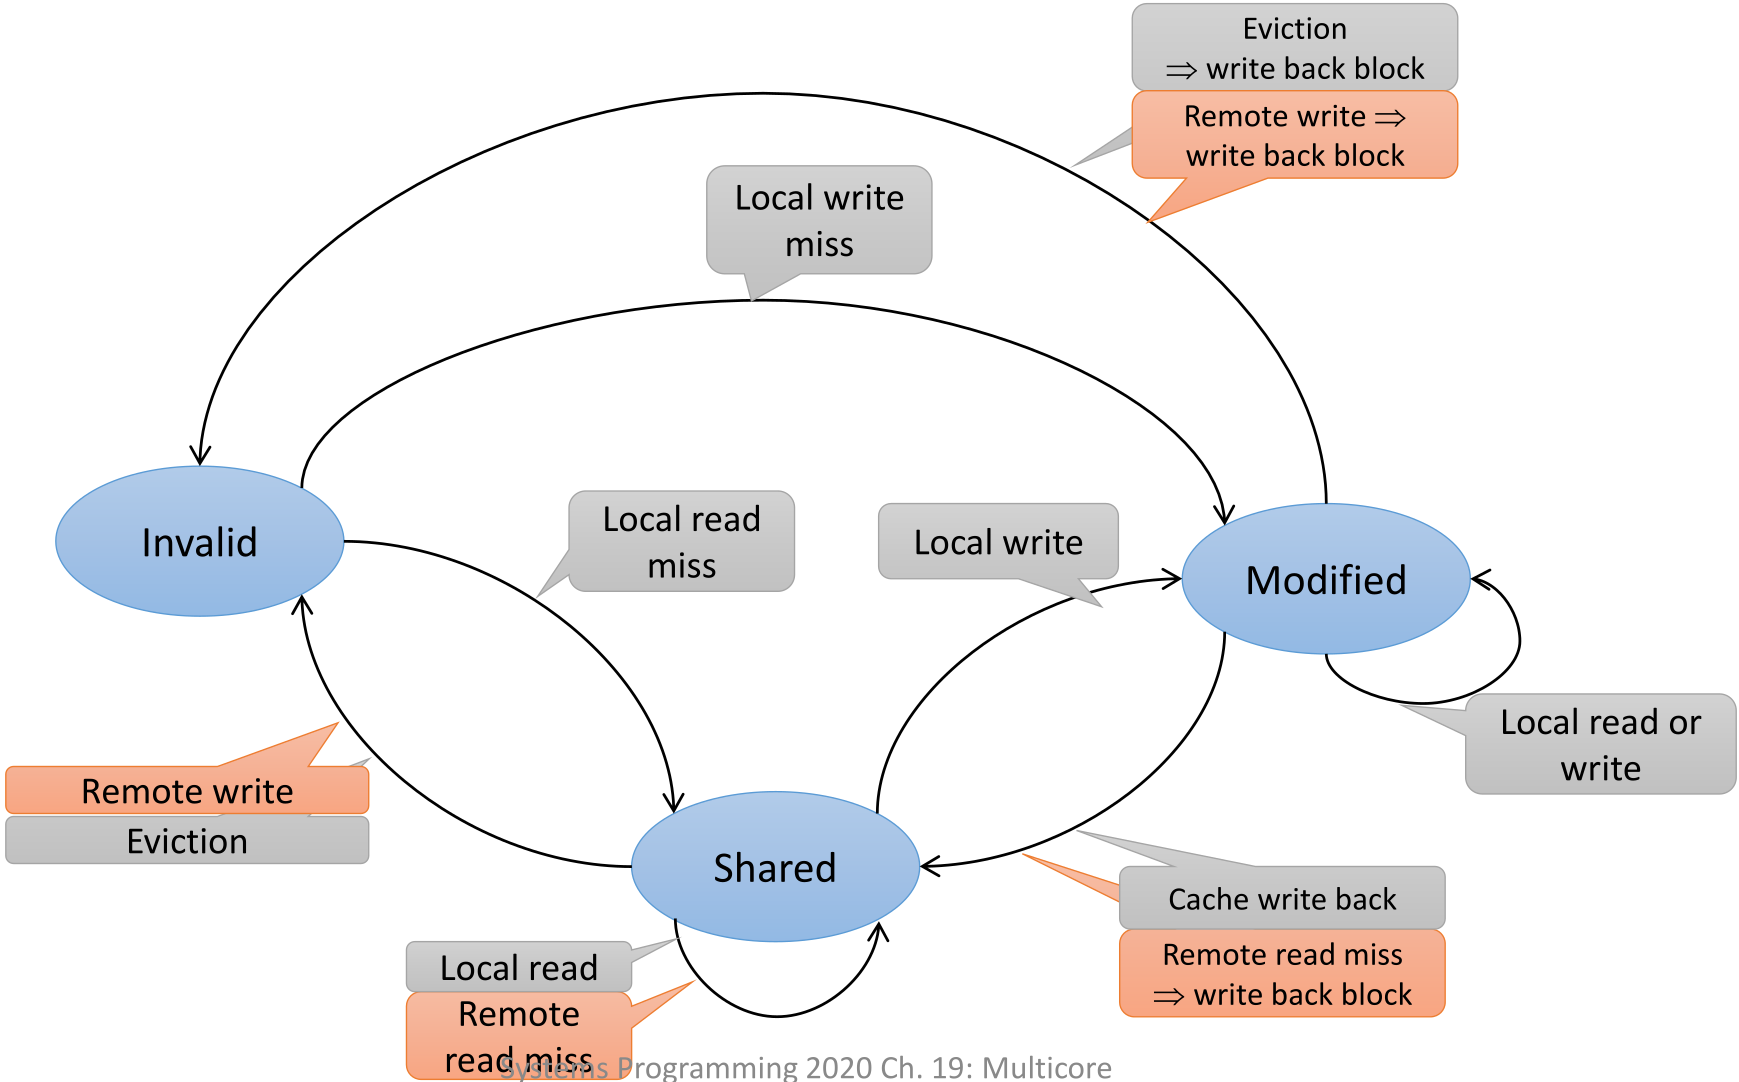
\includegraphics[width=0.8\textwidth]{22_MsiStateTransitions.png}

\paragraph{Issues}
It causes unnecessary bus messages. E.g. if we are in shared and want to write, we first have to check if there are other readers. If we are the only reader, this check is redundant.

Also, the protocol assumes that we are able to distinguish remote processors read and write misses. But in practice this is often not the case. 

\subsubsection{MESI}
Compared to the MSI, it has an additional \textit{Exclusive} state.

The meaning of the states is the following.

When in this state, we know that this is the only copy of this address and the address is clean. 

\begin{itemize}
    \item \textit{Modified}: we have the only copy of this cache block and we have changed the it (it is dirty)
    \item \textit{Exclusive}: we have the only copy of this cache block and it is clean
    \item \textit{Shared}: there may be several copies of this cache block and all are clean
    \item \textit{Invalid}: (same meaning)
\end{itemize}

This protocol also introduces the new bus signal \textit{RdX (Read exclusive)}. If we want to read a cache line and others are reading this block already, we are notified that we read it as \textit{shared}. If there are no other readers, we are notified that we are reading it as \textit{exclusive}. We get this response through the \textit{hit} statement. 

If we hear the RdX signal, it means that another bus is trying to write this block and therefore, we have to invalidate it. 

\paragraph{Invariants}
The MESI invariants are:

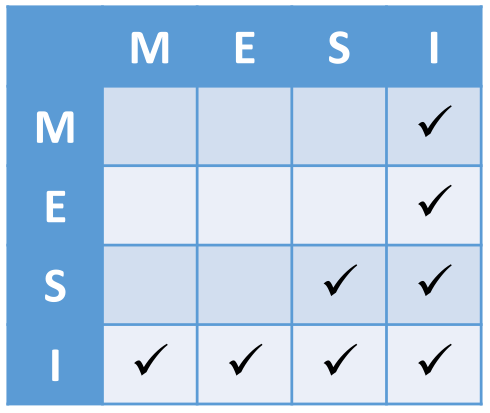
\includegraphics[width=0.8\textwidth]{22_MesiInvariant.png}

The main advantage over MSI is that when we are in exclusive and we want to modify it, we can straight do it without having to notify anyone else.

\paragraph{Transitions}
We can have the following transitions. Grey are local operations by us, orange remote operations by other processors.

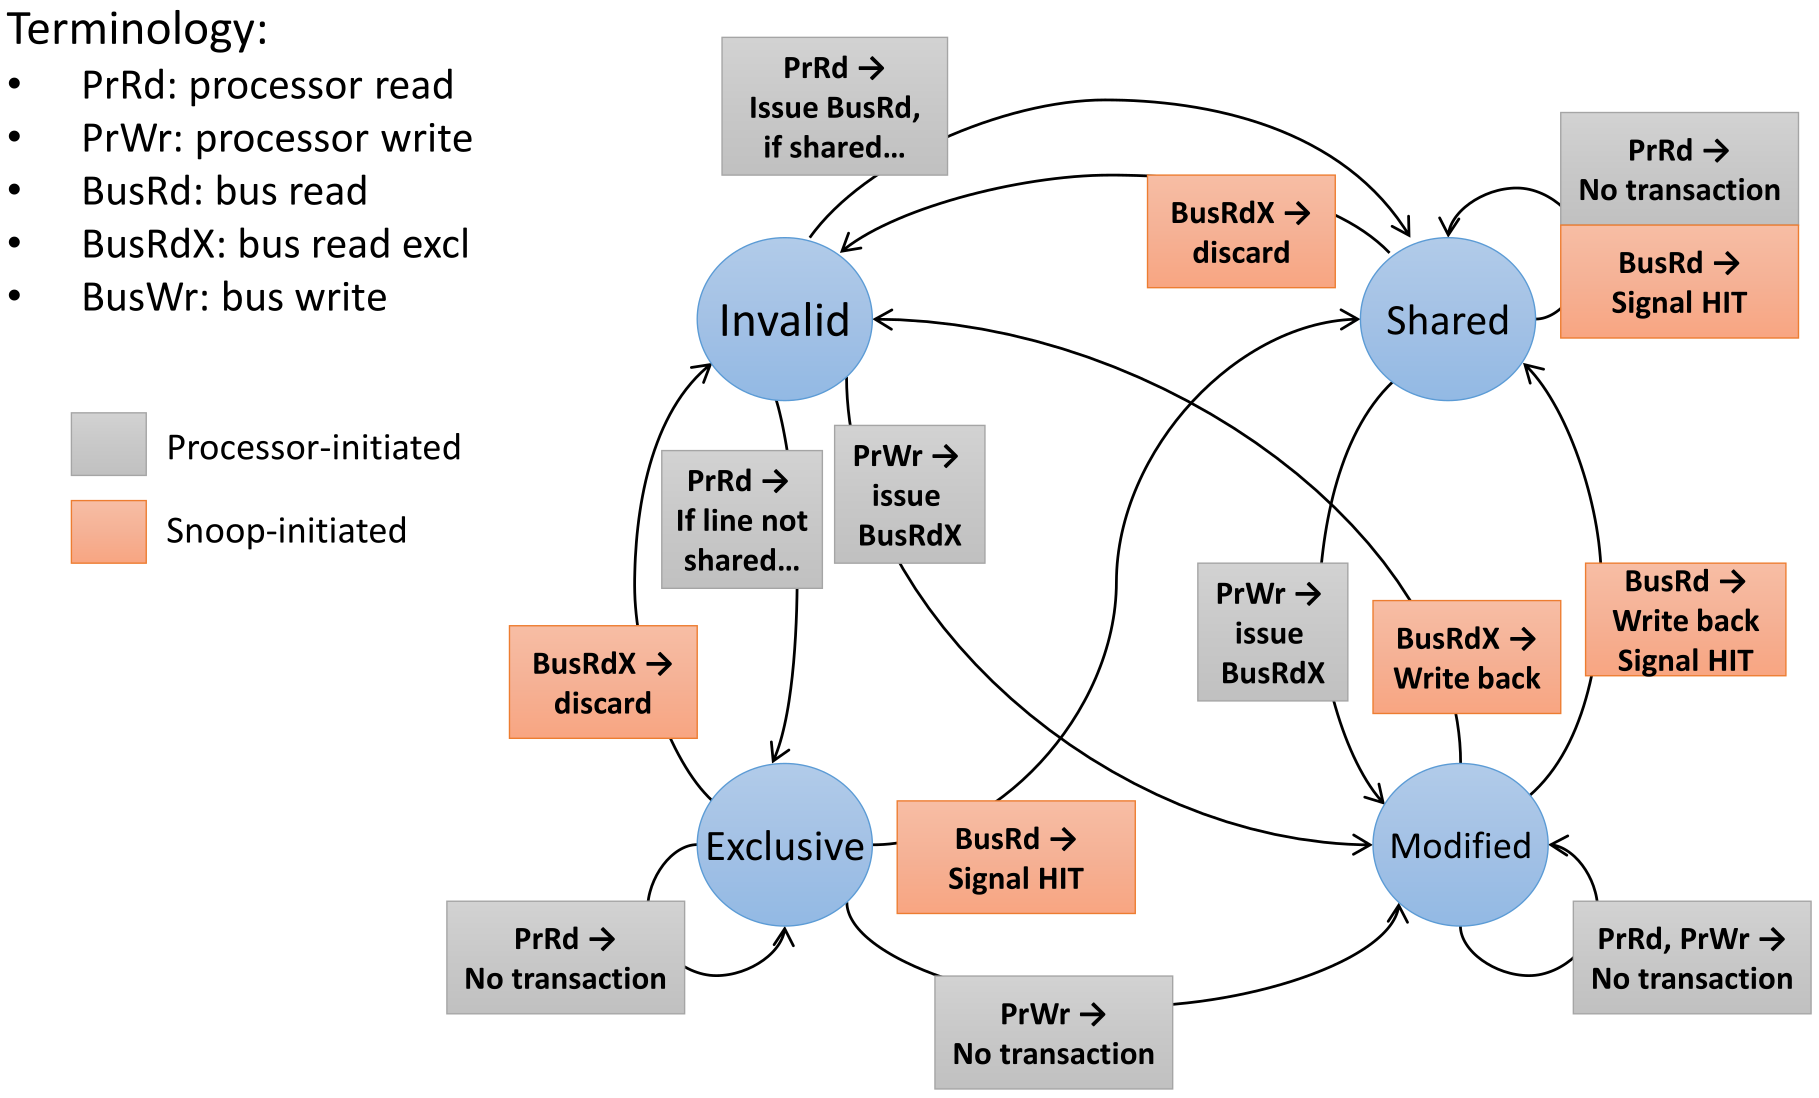
\includegraphics[width=0.8\textwidth]{22_MesiTransitions.png}

\paragraph{Observations}
Data is always first written back to memory, before another process can read it. If data is dirty, we need to write it back to memory. If data is clean, other processes can directly fetch it from main memory. There is no cache-to-cache transfer. So, MESI is good if going to memory is faster than going to remote cache (but often this is not the case).
